\documentclass[MasterThesisMain.tex]{subfiles}
\begin{document}
\chapter{Theory}

\section{Electromagnetic Radiation}
Electromagnetic radiation can be expressed as one dimensional sinusoidal wave using either $\cos$ or $\sin$:

\begin{equation}\label{eq:1dwave}
\varphi = A\sin(Kx-\omega t+\delta),
\end{equation}
where $A$ is the wave amplitude, $K=\frac{2\pi}{\lambda}$ is the propagations number and $\lambda$ is the wave length, angular frequency $\omega = 2\pi\nu$ where $\nu$ is the frequency, time $t$ and initial phase $\delta$.
From electromagnetic theory, the radiation is composed of an electric field and magnetic field that are both perpendicular to the direction of propagation. Both fields can be expressed as one-dimension complex sinusoidal wave. A complex number can be expressed as $C= a + ib =Re(C) + i Im(C) =r\cos(\theta)+ir\sin(\theta)$. Using Eulers formula $\exp(i\theta)=\cos(\theta)+i\sin(\theta)$, the one dimension sinusoidal wave can be expressed as:

\begin{equation}\label{eq:1dcwave}
\varphi=A\cos(\omega t- Kx +\delta) = Re \{A\exp[i(\omega t- Kx +\delta)]\} = A\exp[i(\omega t - Kx + \delta)]
\end{equation}
The wave travels to the right if the phase is $(\omega t - Kx)$ and to the left if the phase is $(\omega t + Kx)$. Changing the order of the first two terms in the phase does not change the propagation of the wave, only the initial phase $\delta$. The wave equation in equation \ref{eq:1dwave} uses $\sin$ in the expression but the complex wave in equation \ref{eq:1dcwave} uses $\cos$, it is the same representation of the wave just moved $2\pi$ in the positive direction. The electric field and magnetic field can be expressed as:

\begin{align}
E=E_0\exp[i(\omega t-Kx+\delta)]\\
B=B_0\exp[i(\omega t-Kx+\delta)]
\end{align}

The relationship between the electric field and magnetic field is given by $E=cB$, and can be derived using the Maxwell-Faraday equation and one dimension wave equations for the electric and magnetic field:

\begin{equation}
\frac{\partial E}{\partial x} = - \frac{\partial B}{\partial t}
\end{equation}

\begin{align}
E = E_0 \cos{(Kx-\omega t)}\\
B = B_0 \cos{(Kx-\omega t)}
\end{align}

Using the Maxwell-Faraday equation the following equation can be formed:

\begin{align}
\frac{\partial E}{\partial x} &= - \frac{\partial B}{\partial t}\\
-K E_0 \sin{(Kx-\omega t)} &= -\omega B_0 \sin{(Kx-\omega t)}\\
E_0 &= \frac{\omega}{K} B_0\\
E_0 &= s B_0
\end{align} 

The constant $\frac{\omega}{K}$ is expressed as the speed $s$ of the light through a medium. In vacuum the speed is equal to the speed of light $s=c$, through a transparent medium the speed is equal to the speed of light divided by the refractive index of the medium $s =\frac{c}{n}$. 

\section{Refractive index} 
Light travelling from one medium to another will undergo change. The speed of the light and the wavelength will change, but not the frequency. The refractive index is a material constant which describes the change and are mostly greater than $1$. The refractive index is defined as:

\begin{equation}
n \equiv \frac{c}{s}
\end{equation}
Where $c$ is the speed of light and $s$ is the speed of light in the medium. The amplitude of the wave will decrease in the medium because the propagations number $K=\frac{2\pi n}{\lambda}$ increases: 

\begin{equation}
E = E_0\exp[i(\omega t - \frac{2\pi n}{\lambda}x + \delta)]
\end{equation}

The change is wavelength is $\lambda = \frac{\lambda_0}{n}$, where $\lambda_0$ is the wavelength before entering the medium. The medium can also absorb light, a term is added to the refractive index to (MISSING WORD) this, and is called the extinction coefficient $k$.

\begin{equation}
N=n-ik
\end{equation}

Placing the complex refractive index into equation \ref{eq:E}, it can be seen that the waves amplitude will decrease exponentially.

\begin{equation}
E = E_0\exp[i(\omega t - \frac{2\pi N}{\lambda}x + \delta)] = E_0\exp(-\frac{2\pi k}{\lambda}x)\exp[i(\omega t - \frac{2\pi n}{\lambda}x + \delta)]
\end{equation}

It needs to be stated that if the phase of the wave is expressed as $(Kx-\omega t)$ and the complex refractive index is given by $N=n-ik$, the exponentially factor will be positive which is incorrect. If the phase of the wave is expressed as $(Kx-\omega t)$ the complex refractive index must be defined as $N=n+ik$.

\section{Reflectance and Transmittance}
When light is reflected upon a surface at an oblique angle, light is reflected and transmitted. Lights electric field is grouped into two oscillation directions which can be defined by two planes, the parallel plane p and the perpendicular plane s. The same applies for lights magnetic field. The parallel plane is defined by the incident and reflected light and the perpendicular plane is perpendicular to the parallel plane. Theory of light regards the two oscillation directions as the p-polarisation and s-polarisation. The reflectance of both p-polarisation and s-polarisation are defined by the ratio of reflected light intensity by the incident light intensity.

\begin{equation}
R_{p} \equiv \frac{I_{r,p}}{I_{i,p}} = \frac{\mid E_{r,p} \mid^2}{\mid E_{i,p} \mid^2} = \mid r_{p} \mid^2 \quad R_{s} \equiv \frac{I_{r,s}}{I_{i,s}} = \frac{\mid E_{r,s} \mid^2}{\mid E_{i,s} \mid^2} = \mid r_{s} \mid^2
\end{equation}

The transmittance can also be expressed using the intensity ratio, $I = n \mid E \mid^2$ and the ratio cross-sectional area for the transmitted and incident ray.

\begin{align}
T_p &\equiv \frac{I_{r,p}\cos(\theta_t)}{I_{i,p}\cos(\theta_i)} = \frac{n_t\cos(\theta_t)}{n_i\cos(\theta_i)}\frac{\mid E_{tp} \mid^2}{\mid E_{ip} \mid^2} = \frac{n_t\cos(\theta_t)}{n_i\cos(\theta_i)} \mid t_{p} \mid^2\\
T_s &\equiv \frac{I_{r,s}\cos(\theta_t)}{I_{i,s}\cos(\theta_i)} = \frac{n_t\cos(\theta_t)}{n_i\cos(\theta_i)}\frac{\mid E_{ts} \mid^2}{\mid E_{is} \mid^2} = \frac{n_t\cos(\theta_t)}{n_i\cos(\theta_i)} \mid t_{s} \mid^2\\
\end{align}

When the extinction coefficient in the refractive index is zero $k=0$, the sum of the reflectance and transmittance is equal to one $R_p + T_p = 1 \quad R_s + T_s = 1 $. If the extinction coefficient is greater than 0 $k>0$, then the sum becomes less than one $R_p + T_p < 1 \quad R_s + T_s < 1 $.	
\section{Fresnel equations for the ambient-substrate model}
Light is reflected and transmitted at the interface of the ambient and substrate\marginpar{Figure and model set up}. The boundary conditions at the interface for the electric and magnetic field\marginpar{Need to understand why B-field is true} in the p-polarisation can be written as:

\begin{align} \label{elbound}
E_{i,p}\cos{(\theta_i)} &= E_{t,p}\cos{(\theta_t)} + E_{r,p}\cos{(\theta_r)}\\
\implies E_{t,p}\cos{(\theta_t)} &= E_{i,p}\cos{(\theta_i)} - E_{r,p}\cos{(\theta_r)}
\end{align} 

\begin{equation} \label{magnbound}
B_{i,p} + B_{r,p} = B_{t,p}
\end{equation}

The subscripts of the electric and magnetic field denote the incident ray $i$, reflected ray $r$ and transmitted ray $t$ in the p-polarisation $p$ plane. The same boundary conditions for the s-polarisation can be expressed. This introduction to the Fresnel equations will use the p-polarisation light. The boundary conditions of the magnetic field need to be reformulated to express the electric field, this is done using the relation $E=cB$. The magnetic field boundary conditions equation \ref{magnbound} can be expressed as:

\begin{align}
\frac{E_{i,p}}{s_i} + \frac{E_{i,p}}{s_i} &= \frac{E_{t,p}}{s_t}\\
\frac{n_i}{c}(E_{i,p}+E_{r,p}) &= \frac{n_t}{c}E_{t,p}\\
n_i(E_{i,p}+E_{r,p}) &= n_tE_{t,p}
\end{align} 

Though the law of reflection the angle of incident is also the angle of reflection $\theta_i=\theta_r$, placing this into the electric field boundary conditions equation \ref{elbound}, the electric field and magnetic field can be expressed as:

\begin{align}
(E_{i,p}-E_{r,p})\cos(\theta_i) &= E_{t,p}\cos(\theta_t) \label{eq:E}\\
\frac{n_i}{n_t}(E_{i,p}+E_{r,p}) &= E_{t,p} \label{eq:B}
\end{align}

Placing equation \ref{eq:B} into equation \ref{eq:E}, the amplitude reflectance coefficient and the reflectance can be calculated for the ambient-substrate system:

\begin{align}
E_{i,p}\cos(\theta_i)-E_{r,p}\cos(\theta_i) &= \frac{n_i}{n_t}(E_{i,p}+E_{r,p}) \cos(\theta_t) \\
E_{i,p}\cos(\theta_i) - \frac{n_i}{n_t}E_{i,p} \cos(\theta_t) &= \frac{n_i}{n_t}E_{r,p} \cos(\theta_t) + E_{r,p} \cos(\theta_i)\\
E_{i,p}(n_t\cos(\theta_i)-n_i\cos(\theta_t)) &= E_{r,p}(n_i\cos(\theta_t)+n_t\cos(\theta_i))\\
r_p = \frac{E_{r,p}}{E_{i,p}} &= \frac{n_t\cos(\theta_i)-n_i\cos(\theta_t)}{n_i\cos(\theta_t)+n_t\cos(\theta_i)} \label{eq:a-srefl}\\
R_p = \mid r_p \mid &^2 
\end{align}

The amplitude transmission coefficient and transmission can be equivalently formulated\marginpar{Complex refractive index fresnel eq can also be expressed}. 

\section{Fresnel equations for the ambient-thin film-substrate model}
The light reflecting and transmitting in this system will interfere both constructive and destructively. To model the optical interference, both the fresnel equation for reflection and transmission will be used:

\begin{align}
r_{jk,p} = \frac{N_k\cos(\theta_j)-N_j\cos(\theta_k)}{N_k\cos(\theta_j)+N_j\cos(\theta_k)} \quad r_{jk,s} = \frac{N_j\cos(\theta_j)-N_k\cos(\theta_k)}{N_j\cos(\theta_j)+N_k\cos(\theta_k)} \\
t_{jk,p} = \frac{2N_j\cos(\theta_j)}{N_k\cos(\theta_j)+N_j\cos(\theta_k)} \quad t_{jk,s} = \frac{2N_j\cos(\theta_j)}{N_j\cos(\theta_j)+N_k\cos(\theta_k)} 
\end{align}

The subscripts denote the reflection and transmission at definite interface. For example $r_{jk,p} = r_{01,p}$, denotes the reflection at the ambient-thin film interface. In the ambient-thin film-substrate model, light at the ambient-thin film interface will be both reflected and transmitted into the layer. The transmitted ray will then be reflected and transmitted at the thin film-substrate interface. The reflected and transmitted phenomenon will proceed through out the thin film. The change in phase at the interface is given by $\exp(-i\beta)$. Figure \ref{fig:beta} represents the ambient-thin film-substrate model, this figure will be used to define the phase variation $\beta$.

The phase of the reflected ray will vary at the the ambient-thin film interface. This variation can be expressed as $K_0\bar{AD}$, where $K_0=\frac{2\pi n_o}{\lambda}$, is the propagation number in air. The phase variation of the transmitted ray is expressed as $K_1(\bar{AB} + \bar{BC})$, where $K_1=\frac{2\pi n_1}{\lambda}$, is the propagation number in the thin film. The length difference can be denoted as $\bar{AB} + \bar{BC} - \bar{AD}$, thus the phase variation of this length difference is:

\begin{equation}\label{eq:phasealpha}
\alpha = \frac{2\pi n_1}{\lambda}(\bar{AB} + \bar{BC}) - \frac{2\pi n_0}{\lambda}\bar{AD}
\end{equation}

Using snells law, $\bar{AD}=\bar{AC}\sin(\theta_0)$ and $\bar{AC}=2d\tan(\theta_1)$ as seen from figure \ref{fig:beta}, this reduces $\bar{AD}$ to:


\begin{align}
\sin(\theta_0) &= \frac{n_1}{n_0}\sin(\theta_1)\\
\bar{AD}&= 2d\frac{\sin(\theta_1)}{\cos(\theta_1)}\sin(\theta_0)\\
\implies \bar{AD}&= 2d\frac{\sin(\theta_1)^2}{\cos(\theta_1)}\frac{n_1}{n_0}
\end{align}


\begin{figure}
\centering
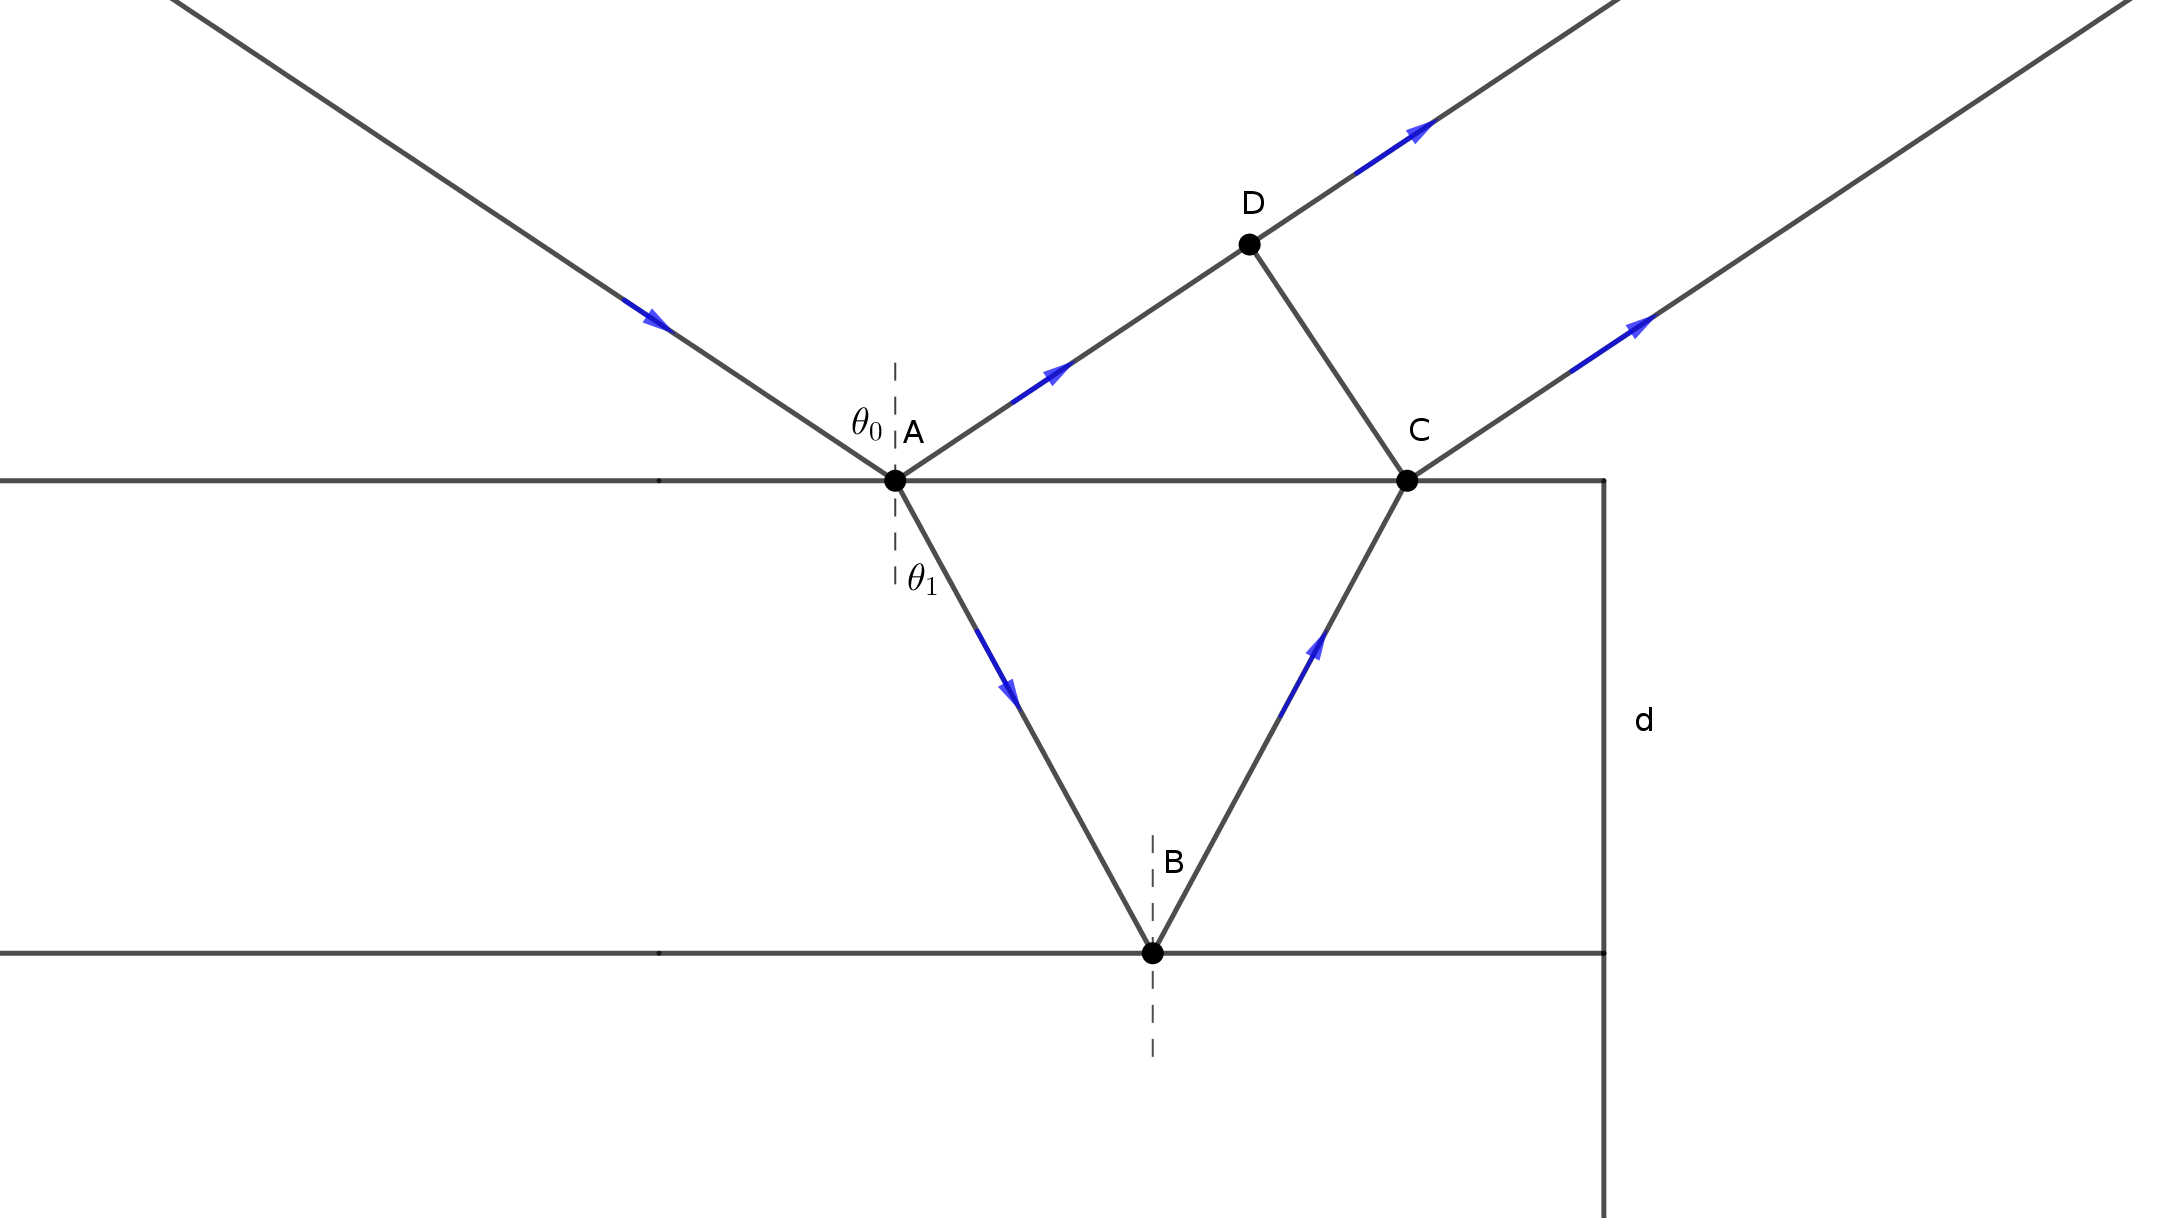
\includegraphics[width=\textwidth]{figbeta.png}
\caption{Light rays from the left will be reflected and transmitted at point A. The reflected light will experience at phase change at point A. The transmitted light will proceed to point B, where it will reflect undergoing a phase change then transmitting at point C. The phase difference between the primary and secondary ray can be calculated by $\alpha = K_1(\bar{AB}+\bar{BC})-K_0(\bar{AD})$}
\label{fig:beta}
\end{figure}  

Inserting this into equation \ref{eq:phasealpha}, and $\bar{AB}=\bar{BC}=\frac{d}{\cos(\theta_1)}$, as seen from figure \ref{fig:beta}, the equation is reduced to:

\begin{align}
\alpha &= \frac{2\pi n_1}{\lambda}\frac{2d}{\cos(\theta_1)}-\frac{2\pi n_0}{\lambda}\frac{2d \sin(\theta_1)^2n_1}{\cos(\theta_0)n_0}\\
&= \frac{4d\pi n_1}{\lambda}\bigg(\frac{1-\sin(\theta_1)^2}{\cos(\theta_1)}\bigg)\\
&= \frac{4d\pi n_1}{\lambda}\cos(\theta_1)
\end{align}

$\alpha$ is the total phase difference of the transmitted beam thus the expression $\alpha=2\beta$ must hold. $\beta$ is called the film phase thickness. \marginpar{$\beta$ can also be expressed in comples ref index.}

\begin{equation}
\beta=\frac{2\pi d}{\lambda} n_1\cos(\theta_1)
\end{equation}  

\begin{figure}
\centering
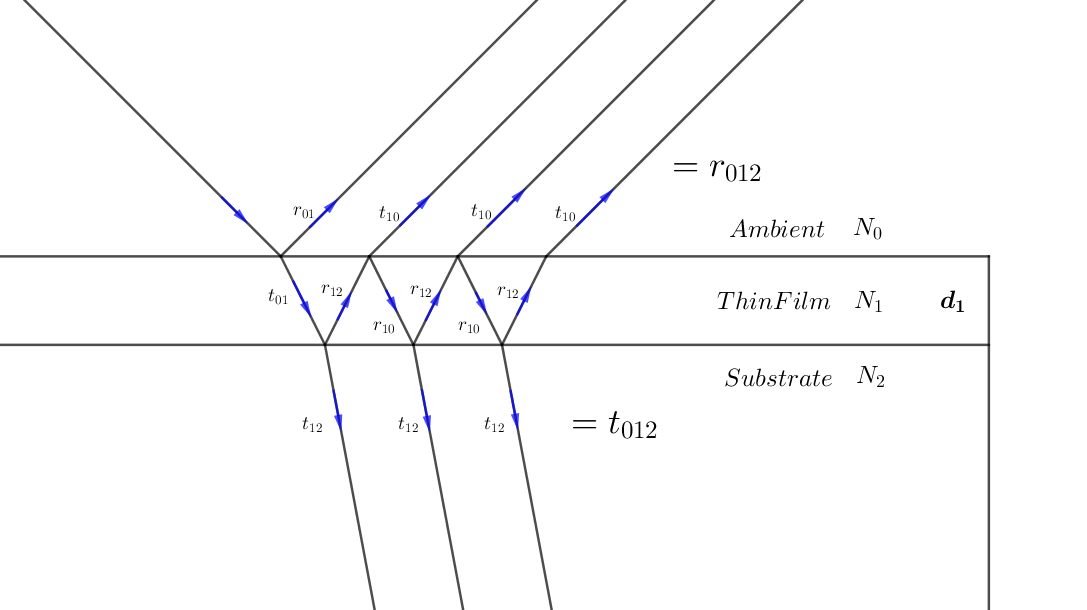
\includegraphics[width=\textwidth]{figrefl.png}
\caption{When light meets an interface, it reflects or transmits. Each light ray is name either reflection $r$ or transmission $t$. Each reflected and transmitted ray is also indexed with two numbers, these denote at which interface the light was reflected or transmitted. A variation of phase happens to each reflected and transmitted rays at every interface. The phase variation at an interface can be expressed by the factor $\exp(-i\beta)$. The primary reflected beam is denoted as $r_{01}$, the second primary reflected beam is denoted $t_{01}r_{12}t_{10}\exp(-i2\beta)$. The reflection amplitude coefficient is the sum of reflected rays that exit the model. The transmission amplitude coefficient is the sum of the transmitted rays that continue into the substrate.}
\label{fig:reflect}
\end{figure}

Using figure \ref{fig:reflect} as a reference the amplitude reflection coefficient can be expressed as the sum of the reflected waves. The first time the ray meets the ambient-thin film interface, the ray will reflect and transmit. The reflected ray $r_{01}$ can be calculated using equation \ref{eq:a-srefl}. The transmitted ray will proceed to the next interface reflect back to the ambient-thin film interface and transmit, giving the second reflected wave in the sum expressed as $t_{01}r_{12}t_{10}\exp(-i2\beta)$. The factor $\exp(-i2\beta)$ comes from the phase difference due to the two interactions at the thin film-substrate interface and thin film-ambient interface. The phase difference factor can be collected multiplied onto the expression since  $\varphi = A\exp(i(\omega t-(Kx+2\beta)+\delta))=A\exp(i(\omega t-(Kx)+\delta))\exp(-i2\beta)$. The total amplitude reflection coefficient can be expressed:

\begin{equation}
r_{012} = r_{01} + t_{01}t_{10}r_{12}\exp(-i2\beta) + t_{01}t_{10}r_{10}r_{12}^2\exp(-i4\beta)+ t_{01}t_{10}r_{10}^2r_{12}^3\exp(-i6\beta)+ \cdots
\end{equation}  
The amplitude reflection coefficient becomes an infinite geometric series which can be reduced using $y=\frac{a}{(1-r)}$, leading to the coefficient being rewritten to:

\begin{equation} \label{eq:r012big}
r_{012}=r_{01}+\frac{t_{01}t_{10}r_{12}\exp(-i2\beta)}{1-r_{10}r_{12}\exp(-i2\beta)}
\end{equation}

The equation \ref{eq:r012big} can be reduced to a more simple equation using $r_{10}=-r_{01}$ and $t_{01}t_{10}=1-r_{01}^2$:

\begin{equation}\label{eq:2layerreflect}
r_{012}= \frac{r_{01}+r_{12}\exp(-i2\beta)}{1+r_{01}r_{12}\exp(-i2\beta)}
\end{equation} 

The following fresnel equation, reflectance and Snell's law for this model are expressed as:

\begin{align}
r_{012,p} = \frac{r_{01,p}+r_{12,p}\exp(-i2\beta)}{1+r_{01,p}r_{12,p}\exp(-i2\beta)} \quad r_{012,s}= \frac{r_{01,s}+r_{12,s}\exp(-i2\beta)}{1+r_{01,s}r_{12,s}\exp(-i2\beta)}\\
t_{012,p} = \frac{t_{01,p}t_{12,p}\exp(-i\beta)}{1+r_{01,p}r_{12,p}\exp(-i2\beta)} \quad t_{012,s} = \frac{t_{01,s}t_{12,s}\exp(-i\beta)}{1+r_{01,s}r_{12,s}\exp(-i2\beta)} \label{eq:2layertrans}
\end{align}

\begin{equation}
R_p=\mid r_{012,p} \mid^2 \quad R_s=\mid r_{012,s} \mid^2
\end{equation}

\begin{equation}
N_0\sin(\theta_0)=N_1\sin(\theta_1)=N_2\sin(\theta_2)
\end{equation} 

\section{Fresnel equations for a multilayer model} 

\begin{figure}
\centering
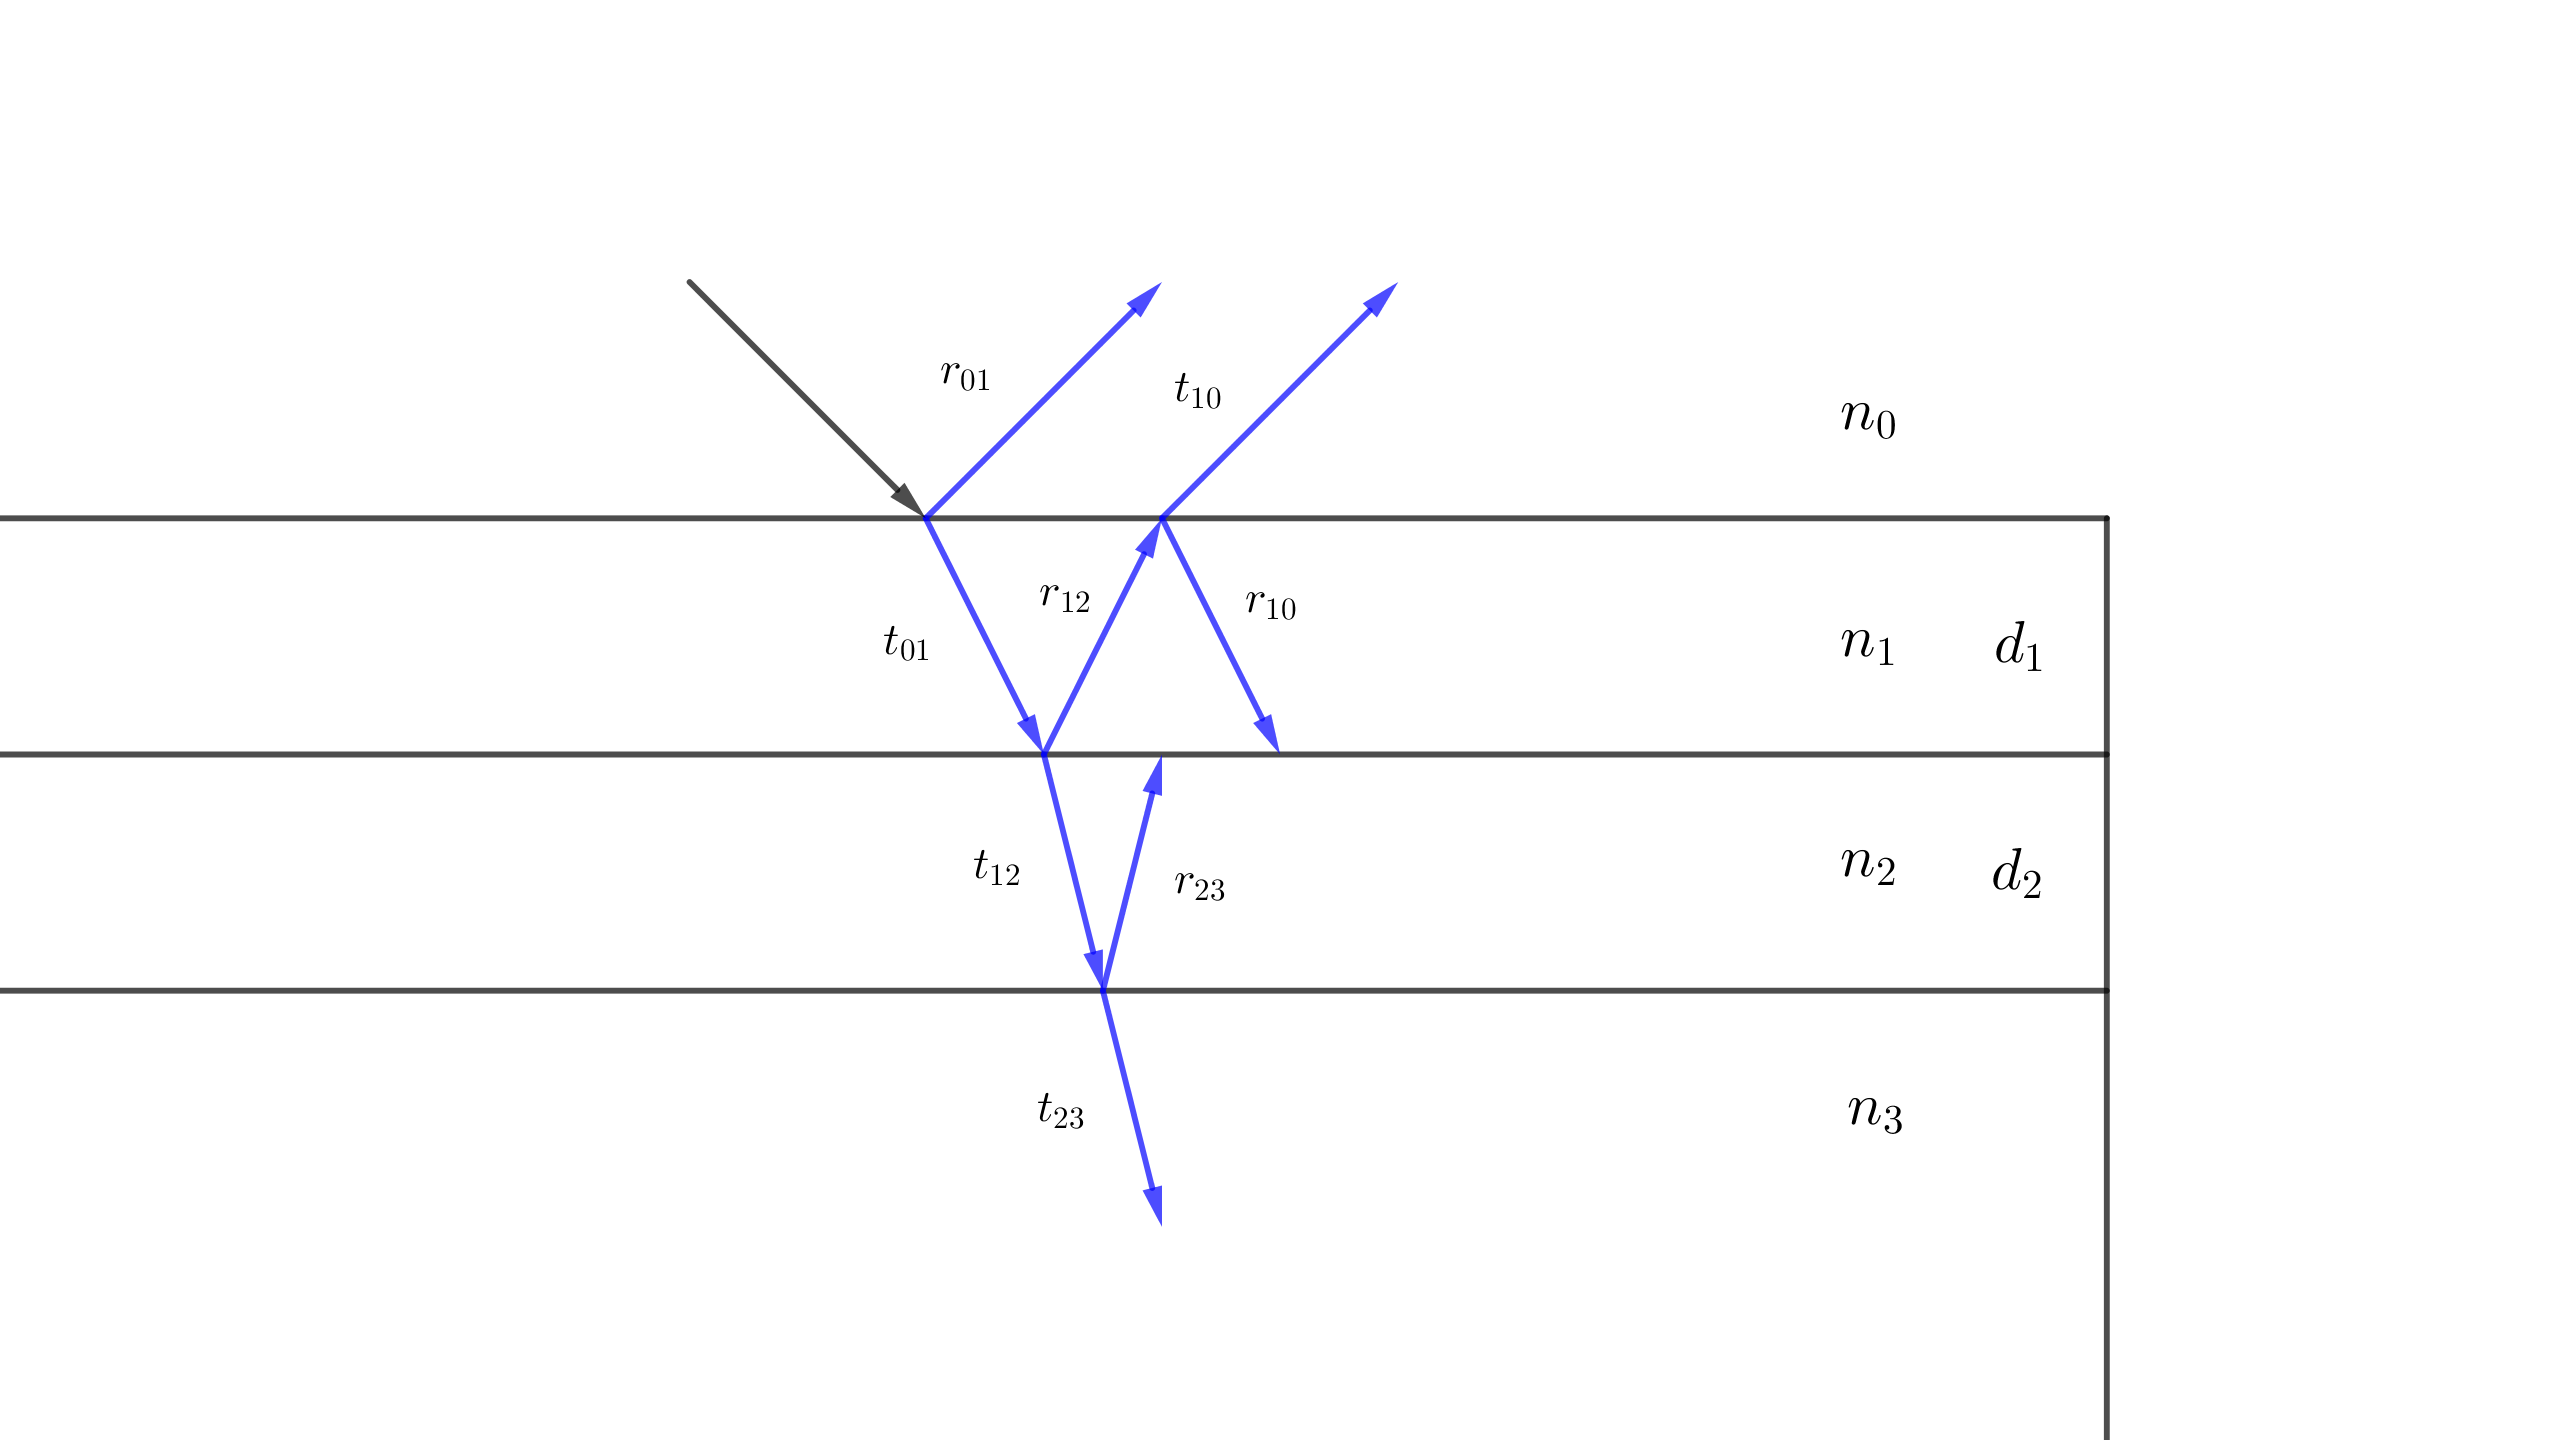
\includegraphics[width=\textwidth]{figmulti1.png}
\caption{The model consists of the ambient,first thin film layer, second thin film layer and substrate. Each layer has a refractive index associated to it and both thin films have a thickness $d_1$ and $d_2$ respectively.}
\label{fig:multilayer1}
\end{figure}

\begin{figure}
\centering
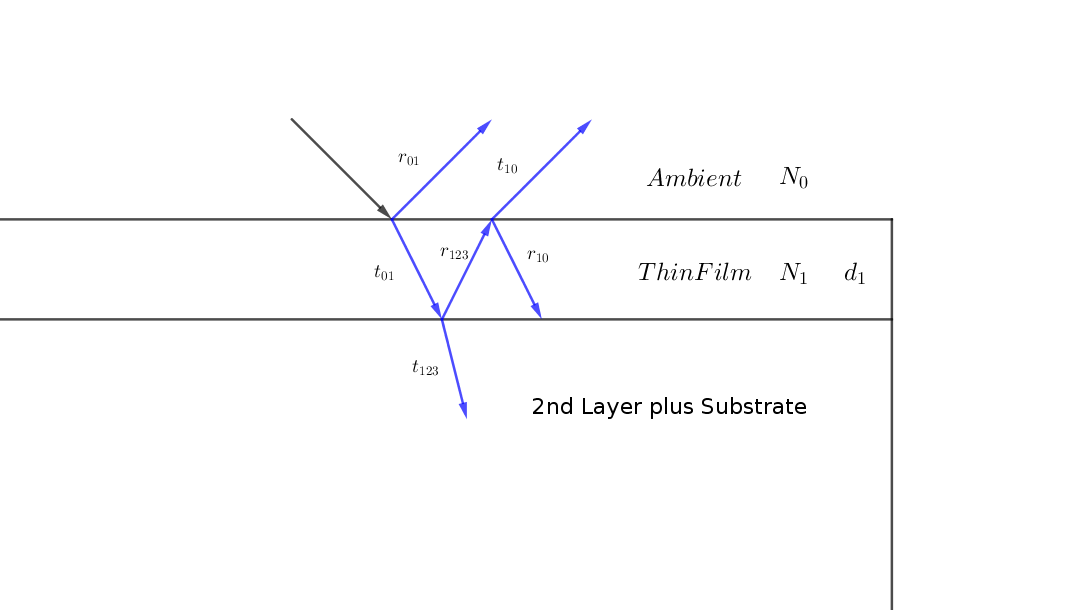
\includegraphics[width=\textwidth]{figmulti2.png}
\caption{The model consists of the ambient,first thin film layer and second thin film layer plus substrate. The second thin film layer and substrate layer has been grouped together because $r_{123}$ and $t_{123}$ has been calculated the model seen in figure \ref{fig:multilayer1} and $r_{0123}$ and $t_{0123}$ can easily be calculated from this model. The ambient and first thin film layer have a refractive index and the first thin film layer has a thickness $d_1$.}
\label{fig:multilayer2}
\end{figure}


In the previous sections, the Fresnel equations for two different models were evaluated. The Fresnel equations for a multilayer model is an amalgamation of the previous models. In an ambient with two thin film layer and substrate model as seen in figure \ref{fig:multilayer1}, the reflection amplitude coefficient $r_{123}$ is calculated, this uses equation \ref{eq:2layerreflect} and the for the transmission amplitude coefficient equation \ref{eq:2layertrans}. These equations produce the following expressions:

\begin{align}
r_{123}= \frac{r_{12}+r_{23}\exp(-i2\beta_2)}{1+r_{12}r_{23}\exp(-i2\beta_2)}\\
t_{123}=\frac{t_{12}t_{23}\exp(-i\beta_2)}{1+r_{12}r_{23}\exp(-i2\beta_2)}
\end{align}

$\beta_2$ is the phase variation in the second thin film layer with thickness $d_2$. This is given as $\beta_2=\frac{2\pi d_2N_2\cos(\theta_2)}{\lambda}$. The substrate and the layer on top of the substrate can be considered as one layer as seen in figure \ref{fig:multilayer2}, thus the reflection amplitude coefficient and transmission amplitude coefficient is expressed as:         

\begin{align}\label{eq:multilayer}
r_{0123}= \frac{r_{01}+r_{123}\exp(-i2\beta_1)}{1+r_{01}r_{123}\exp(-i2\beta_1)}\\
t_{0123}=\frac{t_{01}t_{123}\exp(-i\beta_1)}{1+r_{01}r_{123}\exp(-i2\beta_1)}
\end{align}

Inserting $r_{123}$ and $t_{123}$ into equations \ref{eq:multilayer} the expanded Fresnel equations are expressed for the this multilayer model:

\begin{align}
r_{0123} = \frac{r_{01}+r_{12}\exp(-i2\beta_1)+(r_{01}r_{12}+\exp(-i2\beta_1))r_{23}\exp(-i2\beta_2)}{1+r_{01}r_{12}\exp(-i2\beta_1)+(r_{12}+r_{01}\exp(-i2\beta_1)r_{23}\exp(-i2\beta_2))}\\
t_{0123} = \frac{t_{01}t_{12}t_{23}\exp(-i(\beta_1+\beta_2))}{1+r_{01}r_{12}\exp(-i2\beta_1)+(r_{12}+r_{01}\exp(-i2\beta_1)r_{23}\exp(-i2\beta_2))}
\end{align}
\end{document}